% !TeX TS-program = pdflatex
% !TeX encoding = UTF-8
% !TeX spellcheck = en_GB
% !TeX root = phys.tex
\documentclass[10pt,a4paper,fleqn]{article}
% -------------------------------- %
%\usepackage{lmodern}
\usepackage{cfr-lm}
\usepackage[T1]{fontenc}
\usepackage{textcomp}
\usepackage[utf8]{inputenc}
\usepackage[UKenglish]{babel}
%\hyphenation{}
\usepackage{microtype}
\usepackage{indentfirst}
\usepackage[heightrounded]{geometry}
\usepackage{lipsum}
% -------------------------------- %
% Math
% -------------------------------- %
\usepackage{amsmath}
\usepackage{amssymb}
\usepackage{mathtools}
\usepackage{amsthm}
% -------------------------------- %
\newcommand{\numberset}{\mathbb}
%\newcommand{\N}{\numberset{N}}
\newcommand{\R}{\numberset{R}}
% -------------------------------- %
\renewcommand{\epsilon}{\varepsilon}
%\renewcommand{\theta}{\vartheta}
%\renewcommand{\rho}{\varrho}
\renewcommand{\phi}{\varphi}
% -------------------------------- %
\DeclarePairedDelimiter{\abs}{\lvert}{\rvert}
\DeclarePairedDelimiter{\norma}{\lVert}{\rVert}
\DeclarePairedDelimiter{\set}{\{}{\}}
% -------------------------------- %
\DeclareMathOperator{\sign}{sign}
%\DeclareMathOperator{\Realpart}{Re}
%\renewcommand{\Re}{\Realpart}
\DeclareMathOperator*{\argmax}{arg\,max}
\DeclareMathOperator*{\argmin}{arg\,min}
% -------------------------------- %
% Definitions
\theoremstyle{definition}
\newtheorem{defs}{Definition}
%\newtheorem{propts}{Property}
% Theorems
%\theoremstyle{plain}
%\newtheorem{thm}{Theorem}
%\newtheorem{cor}[thm]{Corollary}
%\newtheorem{prop}{Proposition}
%\newtheorem{lem}[thm]{Lemma}
%\renewcommand{\qedsymbol}{$\blacksquare$}
% Remarks
%\theoremstyle{remark}
%\newtheorem{rmk}{Remark}
% -------------------------------- %
% Numbers
% -------------------------------- %
\usepackage{siunitx}
\sisetup{%
	output-decimal-marker={.},group-separator={\,},%
	%	round-mode=places,round-precision=6,%
	table-parse-only,table-number-alignment=center%
}
% -------------------------------- %
% Tikz and colors
% -------------------------------- %
\usepackage{pgfplots} % + tikz
%\pgfplotsset{/pgf/number format/use comma,compat=newest}
\pgfplotsset{compat=newest}
\usetikzlibrary{calc, topaths}
%\usepackage{tikz} % + graphicx,keyval,xcolor
%\definecolor{Maroon}{cmyk}{0,0.87,0.68,0.32}
\definecolor{RoyalBlue}{cmyk}{1,0.50,0,0}
%\definecolor{halfgray}{gray}{0.55}
\definecolor{webgreen}{rgb}{0,0.5,0}
\definecolor{webbrown}{rgb}{0.6,0,0}
\definecolor{lightergray}{gray}{0.99}

\tikzstyle{treenode} = [draw,circle,minimum width=0.6cm,font=\footnotesize,text centered,
inner sep=1.5pt,outer sep=0pt]
\tikzstyle{graphnode} = [draw,circle,font=\small,minimum width=1.5em,inner sep=0pt,outer sep=0pt,fill=blue!20]
% -------------------------------- %
% Floating objects
% -------------------------------- %
\usepackage{booktabs}
\usepackage{tabularx}
%\usepackage{multirow}
\graphicspath{{./Figures/}, {../py/plots/}}
%\usepackage{subfig}
%\usepackage{wrapfig}
\usepackage{caption}
\captionsetup{format=hang,labelsep=colon,font={small,rm},labelfont={sf,bf}}
%\captionsetup[table]{skip=0.2\medskipamount,position=top}
%\captionsetup[figure]{position=bottom}
\usepackage{flafter}
\usepackage[english,nospace]{varioref}
%\usepackage{enumitem}
% -------------------------------- %
% Code
% -------------------------------- %
%%% ToDo: get the 4everyone
\usepackage[ruled,linesnumbered]{algorithm2e}
\SetNlSty{texttt}{}{}
\SetKw{Or}{or}
\SetKw{And}{and}
\SetKw{Not}{not}
% -------------------------------- %
% Miscellaneous
% -------------------------------- %
\interfootnotelinepenalty=10000
\dimen\footins=2.5cm
\renewcommand{\thefootnote}{\fnsymbol{footnote}}
% -------------------------------- %
% My stuff
% -------------------------------- %
\newcommand{\myTitle}{Travelling Salesman Problem}
\newcommand{\mySubtitle}{}
\newcommand{\mySubject}{Statistical physics and complex systems final project}
\newcommand{\myName}{David Nardi}
\newcommand{\myNameShort}{D. Nardi}
\newcommand{\mySummary}{MSc in Artificial Intelligence}
\newcommand{\myMail}{david.nardi@edu.unifi.it}
\newcommand{\myUrl}{https://github.com/david-inf/Python-TSP}

\newcommand{\omissis}{[\textellipsis\unkern]}
\newcommand{\mail}[1]{\href{mailto:#1}{\texttt{#1}}}
\newcommand{\inToc}[1]%
	{\addcontentsline{toc}{section}{\texorpdfstring{\protect\numberline{}#1}{#1}}}
% -------------------------------- %
\title{\myTitle}
\author{\myName\\ \mySummary\\ \mail{\myMail}\\ \url{\myUrl}}
\date{June 2024}
%\date{2024, June}
% -------------------------------- %
% Page styles
% -------------------------------- %
\usepackage{titleps}
\newpagestyle{main}{% oneside mainmatter
	\sethead[][][]%
	{\slshape\myNameShort}{}{\slshape\myTitle}%
	\setfoot[][][]%
	{}{\thepage}{}}
\newpagestyle{myplain}{% oneside mainmatter
	\sethead[][][]%
	{\slshape\myNameShort}{}{\thepage}%
	\setfoot[][][]%
	{}{}{}}
\usepackage[strict]{changepage}
% -------------------------------- %
% Bibliography
% -------------------------------- %
% Activate bibliography when you are ready
%\usepackage[autostyle,italian=guillemets,babel]{csquotes}
%\usepackage[backend=biber,useprefix,style=ieee,backref,hyperref,defernumbers=true]{biblatex}
%\usepackage[backend=biber,useprefix,style=authoryear-comp,hyperref,defernumbers=true]{biblatex}
%\addbibresource{} % create Db
% -------------------------------- %
\usepackage{hyperref}
\hypersetup{%
	colorlinks,urlcolor=webbrown,linkcolor=RoyalBlue,citecolor=webgreen,%
	linktocpage,pdfstartpage=1,bookmarksnumbered,bookmarksopen,bookmarksopenlevel=2,%
	pdftitle={\myTitle},pdfauthor={\myName},pdfsubject={\mySubject}%
}
% -------------------------------- %
%\usepackage{showframe}
\begin{document}
\frenchspacing
% ************************************************************************************* %
% FRONTMATTER
% ************************************************************************************* %
\cleardoublepage
\pdfbookmark[1]{Title page}{fronte}
\maketitle

\begin{abstract}
With this work we tackle the Travelling Salesman Problem (TSP) using few known algorithms. We start with two local search approaches that swap the edges of the cycle, once we saw that the local searches get trapped in local minima we moved forward to a multi-start meta-heuristic for each local search. Simulated annealing is then tested using a routine to initialize the temperature parameter.

Results show that\dots

Python implementation is available at \href{\myUrl}{this} GitHub repo.
\end{abstract}

\setcounter{tocdepth}{2}
\tableofcontents\cleardoublepage
\pagestyle{main}
% ************************************************************************************* %
% MAINMATTER %
% ************************************************************************************* %
% !TeX spellcheck = en_GB
% ***************************************************** %
\section{Modelling the travelling salesman problem}\label{sc:tsp}
% ***************************************************** %

Given an undirected (weighted) and complete graph $G=(V,E)$, where the set of all nodes $\abs{V}=N$ and the set of all edges $\set{i,j}$ is $\abs{E}=N(N-1)/2$ and their relative cost (weight) $c_{ij}>0$.% An Hamiltonian cycle is a cycle which touches every node in $V$ once and only once, an Hamiltonian cycle might not exist.

We consider the two following layouts (circular and random) with all possible edges and a feasible solution for each one is displayed

\begin{center}
	\begin{minipage}{0.4\textwidth}
		\newcount\mycount
		\begin{tikzpicture}[transform shape]
			\draw [help lines,pink] (-2.5,-2.5) grid (2.5,2.5);% \node[circle,draw,fill=red] at (0,0) {};
			
			\def \n {8}
			\def \radius {2}

			\foreach \i in {1,2,...,\n}{%
				\node[graphnode] (\i) at ({-360/\n * (1 - \i)}:\radius) {\i};
			}

			\def \m {7}
			\foreach \i in {1,2,...,\m}{%
				\mycount=\i
				\advance\mycount by 1
				\foreach \j in {\the\mycount,...,\n}{%
					\draw[-,very thin,gray] (\i) to (\j);
				}
			}

			\foreach \i in {1,...,\m}{%
				\mycount=\i
				\advance\mycount by 1
				\draw[->,very thick] (\i) -- (\the\mycount);
			}
			\draw[->,very thick] (8) -- (1);
		\end{tikzpicture}%\captionof{figure}{Circular layout}
	\end{minipage}\quad
	\begin{minipage}{0.4\textwidth}
		\newcount\mycount
		\begin{tikzpicture}
			\draw [help lines,pink] (-2.5,-2.5) grid (2.5,2.5);% \node[circle,draw,fill=red] at (0,0) {};
			
			\foreach \i/\j in {(0.4,-1.6)/1, (-0.24448624,-0.19845625)/2, (1.8,-0.5168079)/3, (0.78947212,1.70705996)/4, (-1.62329061,0.57546048)/5, (1.90248941,1.29104645)/6, (1.04455881,-0.2263432)/7, (1.14425722,-1.09104511)/8}{%
				\node[graphnode] (\j) at \i {\j};
			}

			\def \n {8}
			\def \m {7}
			\foreach \i in {1,2,...,\m}{%
				\mycount=\i
				\advance\mycount by 1
				\foreach \j in {\the\mycount,...,\n}{%
					\draw[-,very thin,gray] (\i) to (\j);
				}
			}

			\draw[->,very thick] (1) -- (8); \draw[->,very thick] (8) -- (3); \draw[->,very thick] (3) -- (7);
			\draw[->,very thick] (7) -- (4); \draw[->,very thick] (4) -- (6); \draw[->,very thick] (6) -- (5);
			\draw[->,very thick] (5) -- (2); \draw[->,very thick] (2) -- (1);
		\end{tikzpicture}%\captionof{figure}{Random layout}
	\end{minipage}
\end{center}
on the left, a circular graph, for which we know that the optimal solution is a circular path, that is \numlist{1;2;3;4;5;6;7;8} but the same reversed too since the total cost is the same; on the right each node is in a random position, so we don't know exactly the optimal solution, but a good feasible solution can be found in a polynomial time varying with the problem size. % further discussion in the energy view section

We constraint the Hamiltonian cycle to start with the first node 1, so that the total number of possible cycles reduces to $(N-1)!$, a practical trick since we see the cycle as a sequence of all the nodes in the graph.


% ***************************************************** %
\subsection{From an optimization perspective}
% ***************************************************** %
%\looseness=1
The Travelling Salesman Problem (TSP) consists in finding the \emph{shortest Hamiltonian cycle}. The feasible set $F$ is the set of all Hamiltonian cycles in $G$ and the objective function $c(P)$ is the length of the Hamiltonian cycle $P$.

We make use of a logical variable for each edge
\[
x_{ij}=
\begin{cases}
	1 & \text{if $i\rightarrow j$} \\
	0 & \text{otherwise}
\end{cases}
\]
hence the objective function is the sum of all costs associated with the edges in the cycle. This is the \emph{binary} constraint on variables.

Since a feasible solution is a cycle, we must impose the constraint that each node has one incoming and one outgoing edge, that is the \emph{cycle covering} constraint

\begin{center}
	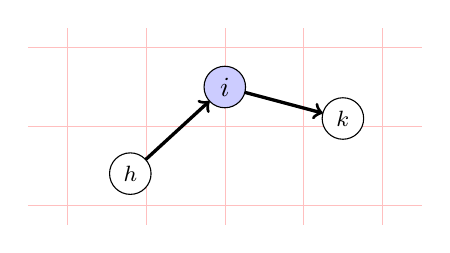
\begin{tikzpicture}
		\draw [help lines,pink] (-2.5,-1.25) grid (2.5,1.25);

		\node[graphnode,fill=white,font=\footnotesize] (h) at (-1.2,-0.6) {$h$};
		\node[graphnode,font=\normalsize] (i) at (0,0.5) {$i$};
		\node[graphnode,fill=white,font=\footnotesize] (k) at (1.5,0.1) {$k$};

%		\draw[->] ($(h)+(15:-0.7)$) -- (h);
		\draw[->,very thick] (h) -- (i); \draw[->,very thick] (i) -- (k);
%		\draw[->] (k) -- ($(k)+(-60:0.7)$);
	\end{tikzpicture}
\end{center}
%that is the \emph{cycle covering} constraint.\par\medskip

Using only this constraint can result in a solution with sub-tours, so we add a constraint for connecting all possible sub-tours

\begin{center}
	\begin{minipage}{0.35\textwidth}
		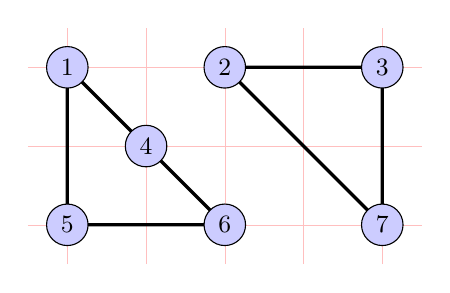
\begin{tikzpicture}
			\tikzset{help lines/.append style=pink}
			\draw [help lines] (-0.5,-1.5) grid (4.5,1.5);% \node[circle,draw,fill=red] at (0,0) {};
			
			%% nodes
			\node[graphnode] (1) at (0,1) {1}; \node[graphnode] (2) at (2,1) {2}; \node[graphnode] (3) at (4,1) {3};
			\node[graphnode] (4) at (1,0) {4};
			\node[graphnode] (5) at (0,-1) {5}; \node[graphnode] (6) at (2,-1) {6}; \node[graphnode] (7) at (4,-1) {7};
			
			%% edges
			\draw[very thick] (1) -- (4) -- (6) -- (5) -- (1);
			\draw[very thick] (2) -- (3) -- (7) -- (2);
			%	\foreach \i in {0,1,...,6}{%
				%		\foreach \j in {0,1,...,6} {%
					%			\draw (\i) -- (\j);
					%		}
				%	}
		\end{tikzpicture}
	\end{minipage}%
	\qquad%
	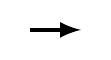
\begin{tikzpicture}
		\draw[-latex,ultra thick] (-0.4,0) -- (0.25,0);
	\end{tikzpicture}%
	\qquad%
	\begin{minipage}{0.31\textwidth}
		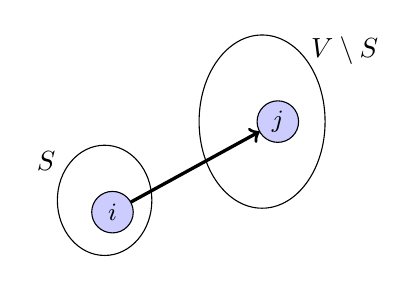
\begin{tikzpicture}
			\draw (0,0) ellipse (0.8 and 1.1); \node[right] at (0.5,0.9) {$V\setminus S$};
			\draw (-2,-1) ellipse (0.6 and 0.7); \node[left] at (-2.5,-0.5) {$S$};
			
			\node[graphnode] (i) at (-1.9,-1.15) {$i$};
			\node[graphnode] (j) at (0.2,0) {$j$};
			
			\draw[->,very thick] (i) -- (j);
		\end{tikzpicture}
	\end{minipage}%\quad\quad%$\Leftarrow$\quad
\end{center}
from a subset $S$ there must be at least an edge to the complementary set $V\setminus S$, the \emph{connection} constraint, the \emph{hard} constraint of the optimization problem.\par\smallskip

The resulting optimization problem will be
\begin{equation}\label{eq:tsp-prob}
	\begin{aligned}
		\min\quad & c(P)=\sum_{\set{i,j}\in E}c_{ij}x_{ij} \\
		& \sum_{\set{i,j}\in E}x_{ij}=2 \\
		& \sum_{i\in S,j\notin S}x_{ij}\geq1\quad\emptyset\subset S\subset V \\
		& x_{ij}\in\set{0,1}
	\end{aligned}
\end{equation}

In practice, for simplicity, the cost for each edge is the Euclidean distance between the two cities, so we can use the distance matrix $D\in\R^{N\times N}$
\[
D=(d_{ij})=
\begin{pmatrix} 
	0 & d_{12} & d_{13} & \cdots & d_{1N} \\
	d_{21} & 0 & d_{23} & \cdots & d_{2N} \\
	d_{31} & d_{32} & 0 & \cdots & d_{3N} \\
	\vdots & \vdots & \vdots & \ddots & \vdots \\
	d_{N1} & d_{N2} & d_{N3} & \cdots & 0
\end{pmatrix}
\]
that is a symmetric matrix, whether an edge is in the cycle or not, the variables $x_{ij}$ become the elements of the adjacency matrix $A$ of the same shape of $D$. The objective function will be $c(P)=A\odot D$ that we call $f(x)$ for simplicity with $x$ a certain solution (sequence); the cycle covering constraint becomes the sum over rows and columns of $A$ that must be equal to $2N$.

%% problem informal description
%Given a list of cities of size $N$ and their relative distances in a matrix , what is the shortest path that visits each city exactly once and returns to the origin city?

%% problem mathematical description

%\begin{align}\label{eq:tsp}
%\min & A\odot D \\
% & \boldsymbol{1}^TA\boldsymbol{1}=1 \\
% & \boldsymbol{1}^TA_Q\boldsymbol{1}\leq\abs{Q}-1
%\end{align}

%\begin{equation}
%\begin{align*}%{lll}
%\min_{a_{ij}} & \sum_{i=1}^N\sum_{\substack{j=1\\i\neq j}}^Nd_{ij}a_{ij} \\
% & \sum_{i=1,i\neq j}^Na_{ij}=1 & i=1,\dots,N \\
% & \sum_{j=1,i\neq j}^Na_{ij}=1 & j=1,\dots,N \\
% & \sum_{\substack{i\in Q}}\sum_{j\in Q,i\neq j}a_{ij}\leq\abs{Q}-1 & \forall Q\subset\set{1,\dots,N},\abs{Q}\geq2
%\end{align*}
%\end{equation}


%\begin{figure}
%\centering
%\begin{tikzpicture} % add adjacency matrix?
%	\tikzset{help lines/.append style=pink}
%	\draw [help lines] (-1,-1) grid (4,2);
%
%	%% nodes
%	\node[graphnode] (0) at (0,0) {0};
%	\node[graphnode] (1) at (1,1.5) {1};
%	\node[graphnode] (2) at (3,1) {2};
%	\node[graphnode] (3) at (2,-0.5) {3};
%
%	%% edges
%	\draw[-stealth] (0) to node[left,font=\small] {$d_{01}$} (1);
%	\draw[-stealth] (1) to node[above,font=\small] {$d_{12}$} (2);
%	\draw[-stealth] (2) to node[right,font=\small] {$d_{23}$} (3);
%	\draw[-stealth] (3) to node[below,font=\small] {$d_{30}$} (0);
%\end{tikzpicture}
%\caption{Example circular disposition}
%\label{fig:tsp-graph}
%\end{figure}


% ***************************************************** %
\subsection{Smoothing the hard constraint, practical TSP}\label{subsc:practical}
% ***************************************************** %

Each one of the algorithms considered starts with a starting feasible solution $x^0$ and then performs a perturbation on that solution in order to find a new neighbouring solution $x^k\rightarrow x^{k+1}$. We can smooth the hard constraint by keeping this solution each time and swapping nodes in the sequence so that the new solution is still an Hamiltonian cycle.

Here we have used two different methods, see figure~\vref{fig:perturbations}, that randomly draw two different nodes $i$ and $j$ given a current solution $x^k$:
\begin{itemize}
	\item \texttt{swap}: given the sequence, swap positions $i$ and $j$, figure~\ref{subfig:swap};
	\item \texttt{reverse}: given the sequence, reverse the position of each nodes between $i$ and $j$ inclusive, figure~\ref{subfig:reverse}.
\end{itemize}


\begin{figure}
\centering
\subfloat[\emph{\texttt{swap} method}\label{subfig:swap}]{%
\begin{tikzpicture}
%	\draw [help lines,pink] (-1,-3) grid (7,2); \node[circle,draw,fill=red] at (0,0) {};
	
	\foreach \i/\j in {1/1,2/5,3/3,4/4,5/2,6/6}{%
		\ifthenelse{\equal{\i}{2}\OR\equal{\i}{5}}{\def\myfill{magenta!20}}{\def\myfill{white}}
		\node[seq point,fill=\myfill] (\i1) at ({\i-0.5},0.5) {\i};
		\node[seq point] (\j2) at ({\j-0.5},-1.5) {\i};
	}
	\node[font=\Large] at ($(11)+(-1,0)$) {$x^k$};
	\node[font=\Large] at ($(12)+(-1,0)$) {$x^{k+1}$};
	
	\draw[-latex,dashed,blue!80,thick] (21.south) -- ++(0,-0.3) -- ($(52.north)+(0,0.3)$) -- (52.north);
	\draw[-latex,dashed,red!80,thick] (51.south) -- ++(0,-0.3) -- ($(22.north)+(0,0.3)$) -- (22.north);
\end{tikzpicture}
}\quad
\subfloat[\emph{\texttt{reverse} method}\label{subfig:reverse}]{%
\begin{tikzpicture}
%	\draw [help lines,pink] (-1,-3) grid (7,2); \node[circle,draw,fill=red] at (0,0) {};
	
	\foreach \i/\j in {1/1,2/5,3/4,4/3,5/2,6/6}{%
		\ifthenelse{\equal{\i}{2}\OR\equal{\i}{5}}{\def\myfill{magenta!20}}{\def\myfill{white}}
		\node[seq point,fill=\myfill] (\i1) at ({\i-0.5},0.5) {\i};
		\node[seq point] (\j2) at ({\j-0.5},-1.5) {\i};
	}
	\node[font=\Large] at ($(11)+(-1,0)$) {$x^k$};
	\node[font=\Large] at ($(12)+(-1,0)$) {$x^{k+1}$};
	
	\draw[latex-latex,dashed,blue!80!red!80,thick] ($(22.north)+(0,0.3)$) -- ($(52.north)+(0,0.3)$);
%	\draw[latex-,dashed,red!80,thick] ($(22.south)+(0,-0.3)$) -- ($(52.south)+(0,-0.3)$);
\end{tikzpicture}
}
\caption{Perturbation methods for generating new solutions. This methods will be used in local search and simulated annealing algorithms.}
\label{fig:perturbations}
\end{figure}











% ************************************************************************************* %
% BACKMATTER %
% ************************************************************************************* %
%\phantomsection
%\inToc{\refname}
%\printbibliography
\end{document}
